\documentclass[11pt,a4paper]{article}
\usepackage[utf8]{inputenc}
\usepackage[T1]{fontenc}
\usepackage{lmodern}
\usepackage[margin=2.4cm]{geometry}
\usepackage{amsmath,amssymb}
\usepackage{booktabs}
\usepackage{graphicx}
\usepackage{xcolor}
\usepackage{microtype}
\usepackage[hidelinks]{hyperref}
\setlength{\parindent}{0pt}
\setlength{\parskip}{6pt}
% Numbers still to be copied from the MATLAB output are marked in red.
\newcommand{\tbd}[1]{\textcolor{red}{#1}}

\begin{document}

\section*{Part A --- Armington with a productivity spillover}

We add to the model of Topic 6 a production spillover, $A_i = \bar A_iL_i^{\lambda}$ with $\lambda\ge 0$ and $\bar A_i$ exogenous; nothing else changes. In the code the spillover is \texttt{par.lambda}, read by \texttt{arm\_solve.m} (line \texttt{Ae = A .* L.\^{}lam}) and by \texttt{arm\_invert.m} (line \texttt{A = Aeff ./ L.\^{}lam}).

% ======================================================================
\subsection*{(a) Equilibrium conditions and identification}

\paragraph{Prices.} Location $i$ produces one variety with labour only, under constant returns and perfect competition, so the price at origin is $w_i/A_i$ and the delivered price in $n$ is $p_{ni}=\tau_{ni}w_i/A_i$ (Topic 6, slide 19). With the spillover,
\begin{equation}
p_{ni}=\frac{\tau_{ni}\,w_i}{\bar A_iL_i^{\lambda}} .
\end{equation}

\paragraph{Price index.} With CES demand and $\phi_{ni}=\tau_{ni}^{1-\sigma}$ (slide 22),
\begin{equation}
P_n^{1-\sigma}=\sum_{i}\phi_{ni}\left(\frac{w_i}{\bar A_iL_i^{\lambda}}\right)^{1-\sigma}
=\sum_i\phi_{ni}\,\bar A_i^{\,\sigma-1}L_i^{\lambda(\sigma-1)}w_i^{1-\sigma}.
\end{equation}

\paragraph{Trade shares.} The share of $n$'s spending on goods from $i$ (slide 21) is
\begin{equation}
\pi_{ni}=\frac{\phi_{ni}\left(w_i/\bar A_iL_i^{\lambda}\right)^{1-\sigma}}
{\sum_k\phi_{nk}\left(w_k/\bar A_kL_k^{\lambda}\right)^{1-\sigma}} .
\end{equation}

\paragraph{Trade balance.} With zero profits the wage bill of $i$ equals the sales of its variety, $w_iL_i=\sum_n\pi_{ni}X_n$ (slide 26). Rents are redistributed to residents, so income per resident is $w_i/\mu$ and spending on goods is $X_n=\mu\,(w_n/\mu)L_n=w_nL_n$ (slide 27). Hence
\begin{equation}
w_iL_i=\sum_n
\frac{\phi_{ni}\left(w_i/\bar A_iL_i^{\lambda}\right)^{1-\sigma}}
{\sum_k\phi_{nk}\left(w_k/\bar A_kL_k^{\lambda}\right)^{1-\sigma}}\;w_nL_n .
\end{equation}
Population now appears on both sides: on the left as the labour force, on the right through productivity, with exponent $\lambda(\sigma-1)$.

\paragraph{$\bar A_i$ and $\lambda$ enter only through $A_i$.} In (2)--(4) $\bar A_i$ and $\lambda$ never appear separately, only in the product $\bar A_iL_i^{\lambda}=A_i$. The remaining conditions do not contain productivity except through $P_n$ and $w_n$: rents $r_i=\frac{1-\mu}{\mu}\frac{w_iL_i}{H_i}$, real utility $W_i=B_i\,(w_i/\mu)/(P_i^{\mu}r_i^{1-\mu})$ (slide 28) and the Fréchet shares $L_i/\bar L=W_i^{\varepsilon}/\sum_sW_s^{\varepsilon}$ (slide 29). So the whole equilibrium depends on $(\bar A,\lambda)$ only through $A$: two parametrizations with the same $\bar A_iL_i^{\lambda}$ in every location are the same economy.

\paragraph{Inversion.} Given data $(L_i,w_i,H_i)$, the matrix $\tau$ and $\sigma$, the inversion of Topic 6 (slides 42--43) solves the trade balance (4) for the competitiveness $c_i=(w_i/A_i)^{1-\sigma}$ by a fixed point, and reads $A_i=w_i\,c_i^{1/(1-\sigma)}$. Since trade shares depend only on ratios of $c_i$, $A$ is recovered up to scale, fixed by a geometric-mean normalization. This step uses $L$ and $w$ as data and never uses $\lambda$: it recovers the composite $A_i$ exactly (\texttt{inv.Aeff}). The fundamental needs $\lambda$:
\begin{equation}
\bar A_i=A_i\,L_i^{-\lambda},
\end{equation}
so it is recovered only for a given $\lambda$ (\texttt{inv.A}).

\paragraph{Every $\lambda$ fits the data equally well.} For any $\lambda'\ge0$ set $\bar A_i(\lambda')=A_iL_i^{-\lambda'}$. Then $\bar A_i(\lambda')L_i^{\lambda'}=A_i$ in every location, so prices, trade shares and the trade balance are those of the true economy, and $(L,w)$ are reproduced exactly. One cross-section gives $N$ equations that pin down $N$ composites; splitting them into $N$ fundamentals and one $\lambda$ requires information the cross-section does not contain. As in Part C of Homework 1, the data identify $A$, not $(\bar A,\lambda)$.

% ======================================================================
\subsection*{(b) The same data inverted with three values of $\lambda$}

\paragraph{What we did.} In \texttt{ARM1\_geography.m} we added a section after act 6. The data are the baseline equilibrium of act 5, generated with $\lambda=0$ (\texttt{par} has no \texttt{lambda} field). We invert them three times, changing $\lambda$ only in a copy of the parameters, so that the data-generating block at the top is untouched:
\begin{verbatim}
p = par;  p.lambda = lam_list(k);          % lam_list = [0 0.07 0.25]
inv = arm_invert(data, p, tau_l, Ltot);
errAeff   = max(abs(log(inv.Aeff ./ Atrue)));
sdAbar(k) = std(log(inv.A));
\end{verbatim}

\begin{table}[h]
\centering
\begin{tabular}{ccc}
\toprule
$\lambda$ & $\max_i|\log(A_i^{\text{inv}}/A_i^{\text{true}})|$ & sd$(\log\bar A_i)$\\
\midrule
0    & $1.17\times10^{-12}$ & 0.3033\\
0.07 & $1.17\times10^{-12}$ & 0.2715\\
0.25 & $1.17\times10^{-12}$ & 0.2041\\
\bottomrule
\end{tabular}
\caption{Same data $(L,w,H)$, three values of $\lambda$ in the inversion. The fixed point converges in 4346 iterations in all three cases; corr$(\log A,\log L)=0.814$, sd$(\log L)=0.575$.}
\end{table}

\paragraph{Why the error on $A_i$ does not depend on $\lambda$.} The composite comes out of the fixed point on the trade balance, which uses only $L$, $w$ and $\tau$: \texttt{lam} enters \texttt{arm\_invert} only after the loop, in \texttt{A = Aeff ./ L.\^{}lam}. So \texttt{inv.Aeff} is the same vector for every $\lambda$ --- same error, $1.17\times10^{-12}$, and even the same number of iterations, 4346 --- and matches the true productivity up to numerical precision (the data were generated with $\lambda=0$, so the true composite equals \texttt{Atrue}). This is point (a) in numbers: the composite is identified.

\paragraph{Why the dispersion of $\log\bar A_i$ does.} The fundamental is $\log\bar A_i=\log A_i-\lambda\log L_i$, so
\begin{equation}
\operatorname{var}(\log\bar A)=\operatorname{var}(\log A)-2\lambda\operatorname{cov}(\log A,\log L)+\lambda^2\operatorname{var}(\log L).
\end{equation}
Productive locations attract people, so $\log A$ and $\log L$ are strongly positively correlated (0.814 here): the larger $\lambda$, the more of the observed productivity is attributed to size and the less to fundamentals, and the fundamentals look more alike. With sd$(\log A)=0.3033$, sd$(\log L)=0.575$ and correlation 0.814, the formula reproduces the table exactly: 0.2715 at $\lambda=0.07$ and 0.2041 at $\lambda=0.25$. The variance falls as long as $\lambda$ is below $\operatorname{cov}(\log A,\log L)/\operatorname{var}(\log L)=0.814\times0.3033/0.575\approx0.43$, the OLS slope of $\log A$ on $\log L$. Same data, same fit, different story about where productivity comes from.

% ======================================================================
\subsection*{(c) The +20\% shock with three values of $\lambda$}

\paragraph{What we did.} We repeat act 5 --- the same fundamentals \texttt{fund3} and the same $+20\%$ shock to $\bar A_j$ in location $j=8$, the middle of the line --- with \texttt{p} in place of \texttt{par} in both calls to \texttt{arm\_solve}. The baseline equilibrium also changes with $\lambda$, because $A_i=\bar A_iL_i^{\lambda}$.

\begin{table}[h]
\centering
\begin{tabular}{cccccc}
\toprule
$\lambda$ & $\Delta L_j$ & $\Delta L_{j-1}$ & $\Delta L_{j+1}$ & $\Delta A_j$ (effective) & $\Delta L_j/\Delta L_j(\lambda{=}0)$\\
\midrule
0    & $+26.91\%$ & $-1.02\%$ & $-0.28\%$ & $+20.00\%$ & 1.00\\
0.07 & $+30.34\%$ & $-1.01\%$ & $+0.03\%$ & $+22.25\%$ & 1.13\\
0.25 & $+45.28\%$ & $-0.69\%$ & $+2.46\%$ & $+31.74\%$ & 1.68\\
\bottomrule
\end{tabular}
\caption{Population change in the shocked location and its two neighbours, and change in its effective productivity $\bar A_jL_j^{\lambda}$.}
\end{table}

\begin{figure}[h]
\centering
\IfFileExists{figures/ARM1_hw2_lambda_shock.png}
  {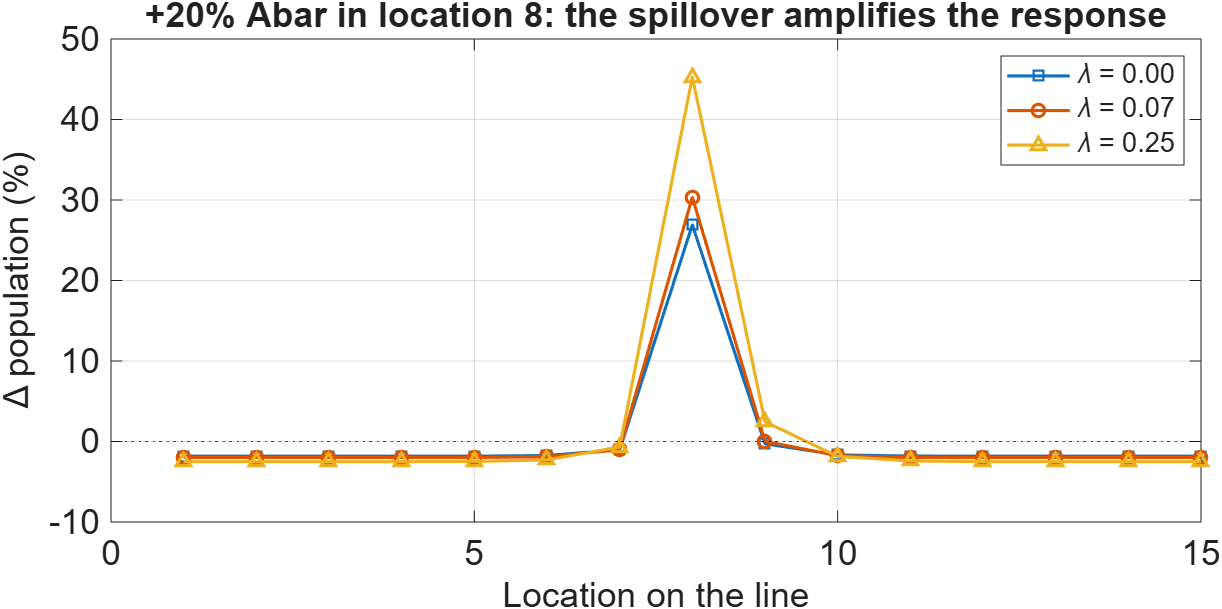
\includegraphics[width=0.85\textwidth]{figures/ARM1_hw2_lambda_shock.png}}
  {\fbox{\parbox{0.8\textwidth}{\centering\tbd{figure ARM1\_hw2\_lambda\_shock.png from the MATLAB run}}}}
\caption{Population change along the line after $+20\%$ $\bar A_j$, for $\lambda=0$, 0.07 and 0.25.}
\end{figure}

\paragraph{Why the response grows with $\lambda$.} The endogenous variable that feeds back into productivity is the population of the shocked location, $L_j$, and it moves through the labour market: workers migrate towards the higher real wage. With $\lambda>0$ they bring productivity with them, since $A_j=\bar A_jL_j^{\lambda}$. The goods market closes the loop: higher $A_j$ lowers the delivered price of $j$'s variety everywhere, its sales and wage bill rise, utility in $j$ rises further and attracts more workers. The last column of the table measures this amplification. The effective productivity obeys an exact identity,
\begin{equation}
1+\Delta A_j = 1.20\,(1+\Delta L_j)^{\lambda},
\end{equation}
so the shock to $\bar A_j$ is $20\%$ in every case, but the productivity the economy actually sees rises by $22.2\%$ at $\lambda=0.07$ ($1.20\times1.3034^{0.07}=1.2225$) and by $31.7\%$ at $\lambda=0.25$ ($1.20\times1.4528^{0.25}=1.3174$). The population response is amplified by a factor 1.13 and 1.68 relative to $\lambda=0$; with $\lambda=0$ we recover exactly act 5 ($+26.906\%$).

\paragraph{The neighbours.} Two forces act on them (slide 39). Migration pulls workers towards $j$; but the neighbours buy a large share of $j$'s variety, now cheaper, so their price index falls and their real wage rises (``proximity protects''). With $\lambda>0$ $j$'s good becomes cheaper still, so the second force is stronger. The table shows it: the left neighbour's loss shrinks from $-1.02\%$ to $-0.69\%$, and the right neighbour goes from $-0.28\%$ to $+0.03\%$ and $+2.46\%$, a gain. The two neighbours differ because their own fundamentals differ (they are drawn at random in act 5). Far from $j$ the price-index gain is small and only the migration pull remains: the farthest locations lose $-1.83\%$ at $\lambda=0$ (act 5) and about $-2.4\%$ at $\lambda=0.25$ (figure). The spillover makes the shock larger and more concentrated in space: the booming location and its neighbours gain more, remote places lose more.

\paragraph{Why it matters for policy.} By point (b) the three values of $\lambda$ fit the same data equally well, yet the same local productivity gain --- a new plant, a subsidy, an infrastructure --- raises the population of the location by $26.9\%$ with $\lambda=0$ and by $45.3\%$ with $\lambda=0.25$. The policy answer depends on a parameter the cross-section cannot identify.

\end{document}
